\chapter{紫外-可见吸收光谱}
\begin{introduction}
    \item 紫外可见光谱及其产生机理
    \item 分子对紫外可见光谱的影响
    \item 紫外可见光谱仪
    \item 紫外可见吸收分析
\end{introduction}
\section{紫外可见光谱及其产生机理}
\subsection{紫外可见光谱}
\begin{definition*}{分子光谱}
    处于气态或溶液中的分子,当发生能级跃迁时,发射或吸收一定频率范围内电磁辐射所组成的带状光谱。
\end{definition*}
\begin{definition*}{紫外-可见吸收光谱法}
    利用紫外-可见分光光度计测量物质对紫外-可见光的吸收程度(即吸光度)或紫外-可见吸收光谱来确定物质的组成、含量等,推理物质结构的分析方法。紫外-可见分光光度法又分为比色法和分光光度法,均属于微量分析。
\end{definition*}
特点:
\begin{itemize}
    \item 灵敏度高,可用于微量组分的测定;
    \item 准确度能满足微量组分测定的要求,相对误差$2\%-5\%$;
    \item 测量仪器相对简单,价格便宜;
    \item 应用广泛,可测定无机物和有机物、可定量或定性分析、可同时测定单一组分或多组分等,还可用于测定络合物的组成、有机酸(碱)及络合物的平衡常数。
\end{itemize}
\subsection{紫外可见光谱的研究对象}
研究对象:在200-380nm的近紫外光区和380-780nm的可见光区有吸收的物质。
\begin{note}
    不能测量<200nm的原因:氧气、氮气、水蒸气存在吸收区,造成严重干扰
\end{note}
\subsection{紫外可见光谱的产生原理}
紫外-可见吸收光谱是由于分子中价电子的跃迁而产生的。
\subsubsection*{有机化合物}
对于有机化合物来说,其分子中存在的电子跃迁有四种:$\pi \rightarrow \pi^{\star},n\rightarrow \pi^{\star},\sigma \rightarrow  \sigma^{\star},n\rightarrow \sigma^{*}$。其中$n\rightarrow\sigma^{*}$能量大,波长短,吸收峰处于远紫外区。在紫外-可见吸收光谱中,可能观测到的跃迁有:
\begin{itemize}
    \item 非共轭体系:所有可能的跃迁中,只有$n\rightarrow n^{*}$的跃迁的能量足够小,相应的吸收光波长在200-800 nm范围内,其他的跃迁能量都太大,它们的吸收光波长均在200 nm以下,无法观察到紫外光谱
    \item 共轭体系:除$n\rightarrow n^{*}$外,还可能有$\pi \rightarrow \pi^{*}$跃迁,它们的吸收光可能落在紫外-可见区。
\end{itemize}
\subsubsection*{无机化合物}
对于无机化合物来说,存在两种跃迁:
\begin{itemize}
    \item 电荷转移跃迁:
    \begin{definition*}{电荷转移跃迁}
        配合物分子吸收辐射后,分子中的电子从主要定域在金属离子M的轨道上转移到配位体L的轨道上或按相反方向转移,这种跃迁叫电荷转移,产生的吸收光谱叫电荷转移光谱。
    \end{definition*}
    \begin{note}
        电荷转移越迁摩尔吸光系数大(>$10^{5}$),可用于定量分析
    \end{note}
    电荷转移越迁有如下三种类型
    \begin{itemize}
        \item $L\rightarrow M$电荷转移:较易还原的金属离子+较易氧化的配体
        \begin{example}
            \ce{TiI4} 紫色,\ce{HgI2}红色,\ce{AgI}黄色,\ce{VO_{4}^{3-}}无色,\ce{CrO_{4}^{2-}}黄色,\ce{MnO_{4}^{2-}}紫色
        \end{example}
        \item $M\rightarrow L$电荷转移:
        \begin{itemize}
            \item 金属离子容易被氧化,如\ce{Ti^{3+}}, \ce{Fe^{2+}},\ce{ V(II)}, \ce{Cu(I)}.
            \item 配体易被还原,具有空位反键轨道,可接受从金属离子中转移的电子:
            \begin{figure}[h]
                \centering
                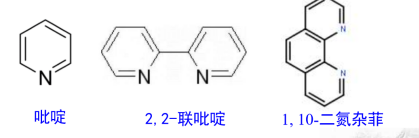
\includegraphics[width=10cm]{image/chp3_L.png}
                \label{fig:chp3L}
                \caption{MM电荷转移示例}
            \end{figure}
        \end{itemize}
        \item $M\rightarrow M$电荷转移:配合物中含有两种不同氧化态的金属离子,电荷在不同氧化态金属离子之间转移。
        \begin{figure}[h]
            \centering
            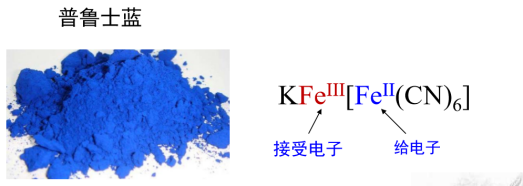
\includegraphics[width=10cm]{image/chp3_MM.png}
            \label{fig:chp3MM}
            \caption{易被还原的配体}
        \end{figure}
    \end{itemize}
    \item 配位场跃迁
    \begin{definition*}{配位场跃迁}
        过渡元素、镧系和锕系元素在真空下,原子、离子的d轨道和f轨道是简并的,在配位体场影响下,简并能级发生分裂成不同能量组轨道,包括d-d跃迁,f-f跃迁。
    \end{definition*}
    \begin{itemize}
        \item d-d跃迁:一些d电子层未充满的第四周期、第五周期的过渡金属元素的吸收光谱,它们的吸收光谱往往比较宽,且容易受环境因素的影响,例如水合铜离子是浅蓝色的,它 的氨络合物是深蓝色的;
        \item f-f 跃迁:大多数镧系和锕系元素的离子在紫外-可见区有吸收,并且吸收峰比较窄。
        \begin{note}
            d-d跃迁的吸收峰较宽,f-f跃迁的吸收峰较窄的原因:
            \begin{itemize}
                \item 外层d电子跃迁时容易受外界环境(溶剂、配位体)的影响
                \item 电子在内层,受外层轨道电子的屏蔽,不易受溶剂、配位体影响。
            \end{itemize}
        \end{note}
    \end{itemize}
\end{itemize}

\section{影响紫外-可见光谱的因素}

\begin{definition*}{生色团}
    在某一段光波内发生吸光的基团,
    \begin{example}
        碳碳共轭结构、含有杂原子的共轭结构、C=O、C=C、C≡C等。
    \end{example}
\end{definition*}
\begin{definition*}{助色团}
    具有非键电子的基团连在双键或共轭体系上,形成非键电子与π电子的共轭,即p-π共轭,使电子活动范围增大,吸收向长波方向位移,使颜色加深的基团。这些基团本身在200nm以上不产生吸收,但这些基团的存在可以增强生色团的生色能力。
    \begin{example}
        $-OH,-OR, -NH_{2}, -NR_{2}, -SR$, 卤素等
    \end{example}
\end{definition*}
\begin{definition*}{红移}
    由于取代基或溶剂的影响,最大吸收峰向长波方向移动的现象称为红移 现象 (red shift)。
\end{definition*}
\begin{definition*}{紫移}
    又叫蓝移(blue shift),是指物质受取代基或溶剂的影响,最大吸收峰向短波方向移动的现象。
\end{definition*}
\begin{definition*}{增色和减色效应}
    指由于化合物结构改变或其他原因,使吸收强度增加(或减弱)的效应,称为增色(减色)效应。
\end{definition*}
\begin{note}
    在吸收光谱中,$\varepsilon $(摩尔吸光系数)值与电子跃迁前后所占据轨道的能差及它们的相互位置有关,轨道间能差越小,分子越处于共平面时,电子的跃迁概率较大,$\varepsilon $值增大,吸收强度增加;反之$\varepsilon$值减小,吸收强度减弱。
\end{note}
\subsection{取代基的影响} 
共轭双键两端有容易使电子流动性增强的基团(给电子基或吸电子基)时,极化现象增强,均使得$\lambda_{max}$红移,$\varepsilon$(摩尔吸光系数)增大。当给电子基与吸电子基同时存在时,产生分子内电荷转移吸收,同样使$\lambda_{max}$红移,$\varepsilon$增大。

\subsection{红移与蓝移}
\begin{itemize}
    \item 共轭效应的影响:$\pi -\pi$共轭,吸收光红移,最大吸收波长由远紫外向近紫外移动;共轭双键数越多,红移越强。
    \begin{itemize}
        \item  π电子共轭体系增大,$\lambda_{max}$红移,$\varepsilon$(摩尔吸光系数)增大;
        \item 空间阻碍使共轭体系破坏,$\lambda_{max}$蓝移,$\varepsilon$(摩尔吸光系数)减小:取代基越大,分子共平面性越差,最大吸收波长蓝移,摩尔吸光系数降低。
    \end{itemize}
    \item 超共轭效应:烃基与$\pi$体系相连,$\pi-\sigma$ 超共轭,紫外吸收红移;连接的烃基基团越大,红移却强。
    \begin{figure}[h]
        \centering
        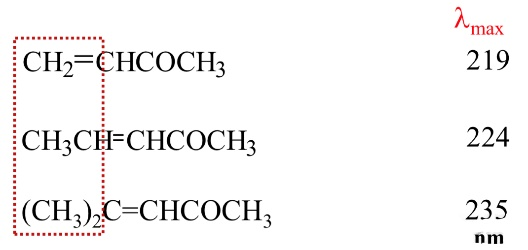
\includegraphics[width=10cm]{image/chp3_ultra.png}
        \label{fig:chp3ultra}
        \caption{超共轭效应}
    \end{figure}
    \item 溶剂的影响:由于受到溶剂和溶质分子间形成氢键、偶极极化等影响,会使溶质吸收波长发生位移:
    \begin{itemize}
        \item 溶剂极性增大时,$\pi \rightarrow \pi^{*}$跃迁吸收带红移,$n\rightarrow \pi^{*}$跃迁吸收带蓝移;
        \item 质子性溶剂容易与吸光分子形成氢键,生色团为质子供体时吸收峰红移,生色团为质子受体时吸收峰蓝移。
    \end{itemize}
\end{itemize}

\subsection{增色与减色效应}

\section{紫外-可见分光光度计}

结构:由光源、单色器、样品室和检测器构成。光从光源发出后,经单色器分光,穿过狭缝进入样品室,最终由检测器接收光信号并转换为电信号。
\begin{itemize}
    \item 光源:提供入射光,要求发射连续的具有足够强度并且稳定的紫外和可见光,辐射强度随波长变化尽可能小,如:钨丝灯(可见光区)、氢灯和氘灯(紫外区);
    \item  单色器:将复合光色散成单色光的光学装置。一般由狭缝、色散元件及透镜系统组成。最常用的色散元件是光栅和棱镜;
    \item  样品室:用于盛放试液的装置,\textcolor{red}{可见光区使用玻璃吸收池},\textcolor{blue}{紫外光区使用石英吸收池};
    \item  检测器:将光信号转变成电信号的装置,如光电管、光电倍增管、光电二极管阵列检测器等。
\end{itemize}
紫外可见光谱仪的分类
\begin{itemize}
    \item 单光束分光光度计:
    \begin{figure}[h]
        \centering
        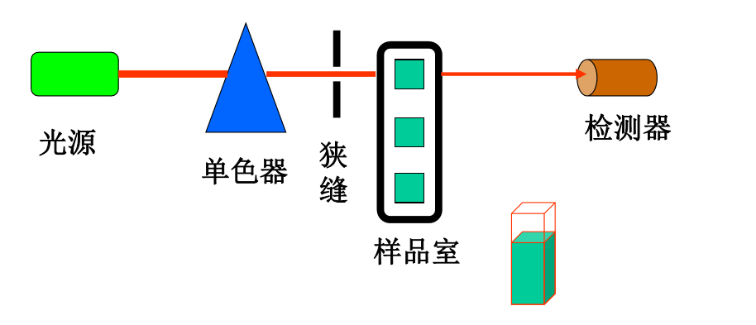
\includegraphics[width=10cm]{image/chp3_single_beam.png}
        \label{fig:chp3singlebeam}
        \caption{单光束分光光度计}
    \end{figure}
    \begin{note}
        单光束光度计缺点:
        \begin{itemize}
    \item  操作麻烦,需扣除背景;
    \item  不能进行吸收光谱的自动扫描;
    \item  光源不稳定性影响测量精密度。
\end{itemize}
    \end{note}
    \item 双光束分光光度计:
    \begin{itemize}
        \item  单波长双光束分光光度计
        \begin{figure}[h]
            \centering
            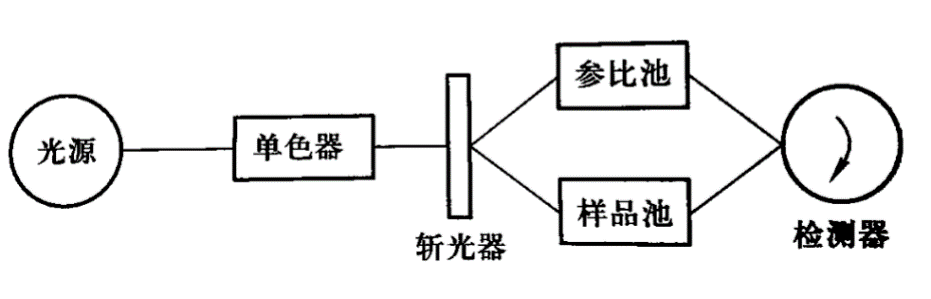
\includegraphics[width=10cm]{image/chp3_single_wl.png}
            \label{fig:chp3singlewl}
            \caption{单波长双光束分光光度计}
        \end{figure}
        
        从光源发出的光经分光后分成两束,交替通过参比池和样品池,测得的是透过样品溶液和参比溶液的光信号强度之比,克服了光源不稳定引起的误差,实现了对全波段、快速自动吸收光谱扫描。
        \item 双波长双光束分光光度计
        \begin{figure}[h]
            \centering
            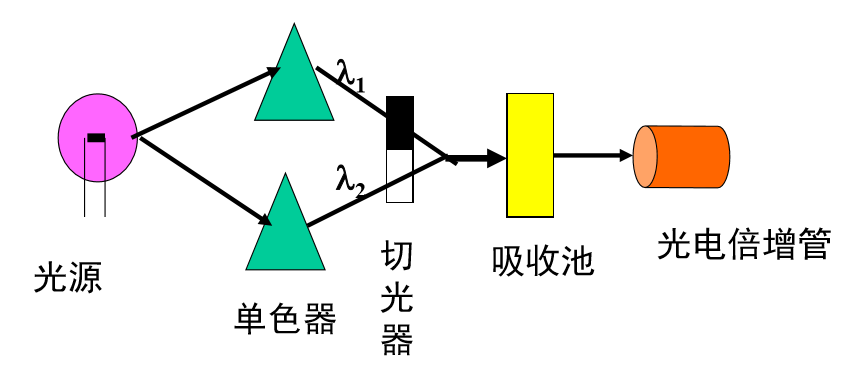
\includegraphics[width=10cm]{image/chp3_double_wl.png}
            \label{fig:chp3doublewl}
            \caption{双波长双光束分光光度计}
        \end{figure}
        
        可消除光谱重叠干扰和背景干扰,主要特点是可以降低杂散光,光谱精度高。
    \end{itemize}
\end{itemize}
\section{紫外可见吸收光谱}
\subsection{紫外可见吸收分析的定量基础}
\begin{theorem*}{朗伯比尔定律}
    当一束平行单色光垂直通过某一均匀非散射的吸光物质时,其吸光度A与吸光物质的浓度c及吸收层厚度b成正比,而与透光度T呈反相关
    \begin{equation*}
        A=\varepsilon bc =lg(\frac{1}{T})
    \end{equation*}
\end{theorem*}
\begin{note}
$A$:吸光度,无量纲

$\varepsilon$:摩尔吸光系数,指的是浓度为1 mol/L的物质在1cm厚的吸收池内产生的吸光度,单位为L/(mol·cm);

$b$:液层厚度,单位为cm;

$c$:溶液中吸光物质的浓度,单位为mol/L。
\end{note}

吸收定律的性质:
\begin{itemize}
    \item 吸收定律具有加和性:如果某一试液中多个组分对同一波长的光有吸收作用,则总吸光度等于各组分的吸光度之和;
    \item 吸收定律只适合单色光:描述吸光度值时需说明光源的波长;
    \item 吸收定律因化学反应而偏离:因解离、络合等原因,待测物质并不都以能对特定频率辐射进行有效吸收的形态存在,可能导致吸收定律结果的偏离。
\end{itemize}

\subsection{紫外-可见吸收光谱的误差}
\begin{itemize}
    \item  溶液偏离朗伯-比尔定律所引起的误差:
    \begin{figure}[h]
        \centering
        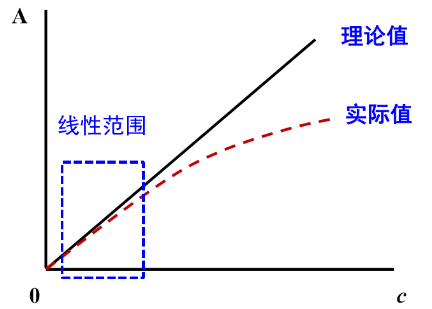
\includegraphics[width=6cm]{image/chp3_billlaw_offset.png}
        \label{fig:chp3offset}
        \caption{溶液偏离朗伯-比尔定律}
    \end{figure}
采用工作曲线的直线段测定待测溶液浓度。减少由入射光为非单色光所引起的误差。利用试剂空白以及确定适宜的浓度范围来减少溶液本身所引起的误差。
    \item  仪器误差:
    \begin{itemize}
        \item 机械系统:吸收池的质量,检流计的灵敏度;
        \item 光学系统:光源不稳定,棱镜的性能,光电管质量等。
    \end{itemize}
    \item  操作误差:由所采用的实验条件与正确的条件有差别引起,
    如:显色条件和测量条件掌握不够好。
\end{itemize}

\subsection{紫外-可见吸收光谱测量条件的选择}
\begin{itemize}
    \item 入射光波长的选择:
    
    以最大吸收波长为入射光波长。此处波长的吸光系数最大,测定的灵敏度更高,且此处波长处吸光度有一小的平坦区,能减少和消除由于单色光的不纯而引起的对朗伯-比尔定律的偏移,从而提高测定的准确度。
    
    \item 吸光度读数范围的选择:
    \begin{equation*}
        \frac{\Delta c}{c}=\frac{0.434}{T log T}\Delta T
    \end{equation*}
    透射率T为$20\%-65\%$时,测量误差<2$\%$。
    可通过控制溶液的浓度来控制透射率。
    
    \item 参比溶液的选择:
     \begin{itemize}
        \item 纯溶剂空白:当试液、试剂、显色剂均为无色时,可直接用纯溶剂(或蒸 馏水)作为参比溶液;
        \item  试剂空白:试液无色,而试剂或者显色剂有色时,可在同一显色反应条件下,加入相同量的显色剂和试剂,稀释同一体积,以此作为参比溶液;
        \item  试液空白:试剂和显色剂均为无色,试液中其他离子有色时,可采用不加显色剂的试液作为参比溶液。
    \end{itemize}

\end{itemize}    